% Set the document class and theme
\documentclass{beamer}

\usetheme{Madrid}
\useoutertheme{miniframes} % Alternatively: miniframes, infolines, split
\useinnertheme{circles}

\definecolor{IITHorange}{RGB}{243, 130, 33} % UBC Blue (primary)
\definecolor{IITHyellow}{RGB}{254, 203, 10} % UBC Grey (secondary)

\setbeamercolor{palette primary}{bg=IITHorange,fg=white}
\setbeamercolor{palette secondary}{bg=IITHorange,fg=white}
\setbeamercolor{palette tertiary}{bg=IITHorange,fg=white}
\setbeamercolor{palette quaternary}{bg=IITHorange,fg=white}
\setbeamercolor{structure}{fg=IITHorange} % itemize, enumerate, etc
\setbeamercolor{section in toc}{fg=IITHorange} % TOC sections

% Override palette coloring with secondary
\setbeamercolor{subsection in head/foot}{bg=IITHyellow,fg=white}

\setbeamertemplate{caption}[numbered]
\setbeamertemplate{theorems}[numbered]

\usepackage{./presentation_macros}

\title[Cryptanalysis of DES]{CS5760: Cryptanalysis of DES and DES-like Iterated Cryptosystems}
\date{February 3, 2025}
\author{Gautam Singh}
\institute[IITH]{Indian Institute of Technology Hyderabad}

\begin{document}
    
    \begin{frame}
        \titlepage
    \end{frame}
    
    \begin{frame}
        \tableofcontents
    \end{frame}
    
    \section{Introduction}
    \label{sec:intro}
    
    \begin{frame}
        \frametitle{Differential Cryptanalysis}
        \begin{columns}
            \begin{column}{0.65\textwidth}
                \begin{enumerate}
                    \item<1-> Chosen plaintext attack.
                    \item<1-> Exploit XOR between plaintext pairs to find key bits.
                    \item<2-> Per DES round, XOR of respective inputs is:
                    \begin{itemize}
                        \item \emph{Linear} in expansion \(E\) to get \(S_E\).
                        \item \emph{Invariant} in key mixing with subkey \(S_K\)
                        to get \(S_I = S_E \oplus S_K\).
                        \item \emph{Linear} in permutation \(P\) on \(S_O\)
                        after S boxes.
                        \item \emph{Invariant} in XOR operation connecting
                        rounds.
                    \end{itemize}
                    \item<3-> S boxes are \emph{nonlinear}. Probability analysis
                    performed between input and output XOR.
                \end{enumerate}
            \end{column}
            \begin{column}{0.35\textwidth}
                \begin{figure}[!ht]
                    \centering
                    \includegraphics<2->[width=\columnwidth]{images/des_f.png}
                    \only<2->{\caption{\(F\) function of DES.}}
                    \label{fig:des-f}
                \end{figure}
            \end{column}
        \end{columns}
    \end{frame}

    \section{Preliminaries}    
    \label{sec:prelims}

    \subsection[S Boxes]{Probability Analysis of S Boxes}
    \label{subsec:s-boxes}
    
    \begin{frame}
        \frametitle{Probability Analysis of S Boxes}
        \begin{enumerate}
            \item Suppose \(Si_I^\prime = Si_I \oplus Si_I^*\) is the input XOR
            to the \(i\)\textsuperscript{th} S box, and \(Si_O^\prime\) is the
            output XOR (\(1 \le i \le 8\)).
            \item<2-> We create a \emph{pairs XOR distribution table} for each S
            box.
            \begin{itemize}
                \item Each entry \(\brak{Si_I^\prime, Si_O^\prime}\) equals the
                number of 6-bit key blocks \(Si_K\) for which \(Si_I^\prime
                \rightarrow Si_O^\prime\).
                \item 64-by-16 joint probability mass function.
            \end{itemize}
            \item<3-> This joint PMF can reduce the number of possible
            (sub)keys. Used to drive choice for the plaintext XOR.
            \begin{itemize}
                \item \(\approx 80\%\) entries are non-zero/possible for each S
                box (some have lesser percentages).
                \item Given \(Si_I^\prime\) and \(Si_O^\prime\), we can narrow
                down \(Si_K\) to a few possibilities.
            \end{itemize}
            \item<4-> \(i\)\textsuperscript{th} S box contributes probability
            \(p_i\) for \(Si_I^\prime \rightarrow Si_O^\prime\). 
            \begin{itemize}
                \item For \(X \rightarrow Y\) over a round, \(P = \prod_i p_i\).
                \item Over \(n\) rounds, \(P = \prod_{i=1}^n P_i\).
            \end{itemize}
            \only<5->{\bfseries Desirable for cryptanalysis: high \(P\) with
            large \(n\).}
        \end{enumerate}
    \end{frame}

    \subsection{Characteristic}
    \label{subsec:char}

    \begin{frame}
        \frametitle{Characteristic}
        \begin{definition}[Characteristic]
            An \emph{n-round chracteristic} is a tuple \(\Omega =
            \brak{\Omega_P, \Omega_\Lambda, \Omega_T}\) where \(\Omega_P =
            \brak{L^\prime, R^\prime}\) and \(\Omega_T = \brak{l^\prime,
            r^\prime}\) are \(m\) bit numbers, \(\Omega_\Lambda =
            \brak{\Lambda_1, \ldots, \Lambda_n}\), \(\Lambda_i =
            \brak{\lambda_I^i, \lambda_O^i}\) and \(\lambda_I^i,
            \lambda_O^i, L^\prime, R^\prime, l^\prime, r^\prime\) are
            \(\frac{m}{2}\) bit numbers and \(m\) is the block size of the
            cryptosystem satisfying
            \begin{align}
                \lambda_I^1 &= R^\prime \\
                \lambda_I^2 &= L^\prime \oplus \lambda_O^1 \\
                \lambda_I^n &= r^\prime \\
                \lambda_I^{n-1} &= l^\prime \oplus \lambda_O^n \\
                \forall\ 1 < i < n,\ \lambda_O^i &= \lambda_I^{i-1} \oplus \lambda_I^{i+1}
                \label{eq:char-def}
            \end{align}
        \end{definition}
    \end{frame}

    \begin{frame}
        \frametitle{Characteristic}
        \begin{definition}[Right Pair]
            A \emph{right pair with respect to an n-round characteristic
            \(\Omega = \brak{\Omega_P, \Omega_\Lambda, \Omega_T}\) and an
            independent key \(K\)} is a pair for which \(P^\prime = \Omega_P\)
            and for each round \(i\) of the first \(n\) rounds of the encryption
            of the pair using \(K\) the input XOR of the
            \(i\)\textsuperscript{th} round equals \(\lambda_I^i\) and the
            output XOR of the \(F\) function equals \(\lambda_O^i\). Pairs that
            do not satisfy these conditions are called \emph{wrong pairs}.
        \end{definition}
        \pause
        \begin{definition}[Probability of a Round of a Characteristic]
            Round \(i\) of an \(n\)-round characteristic \(\Omega\) has
            probability \(p_i^\Omega\) if \(\lambda_I^i \rightarrow
            \lambda_O^i\) with probability \(p_i^\Omega\) by the \(F\) function.
        \end{definition}
    \end{frame}

    \begin{frame}
        \frametitle{Probability of a Characteristic}
        \begin{definition}[Probability of a Characteristic]
            An \(n\)-round characteristic \(\Omega\) has probability
            \(p^\Omega\) given by
            \begin{equation}
                p^\Omega = \prod_{i=1}^n p_i^\Omega
                \label{eq:prob-char}
            \end{equation}
        \end{definition}
        \pause
        \begin{theorem}[Probability of a Characteristic and Right Pairs]
            The formally defined probability of a characteristic \(\Omega =
            \brak{\Omega_P, \Omega_\Lambda, \Omega_T}\) is the probability that
            any fixed plaintext pair satisfying \(P^\prime = \Omega_P\) is a
            right pair when random independent keys are used.
        \end{theorem}
    \end{frame}

    \begin{frame}
        \frametitle{Example of a Characteristic}
        \begin{figure}[!ht]
            \centering
            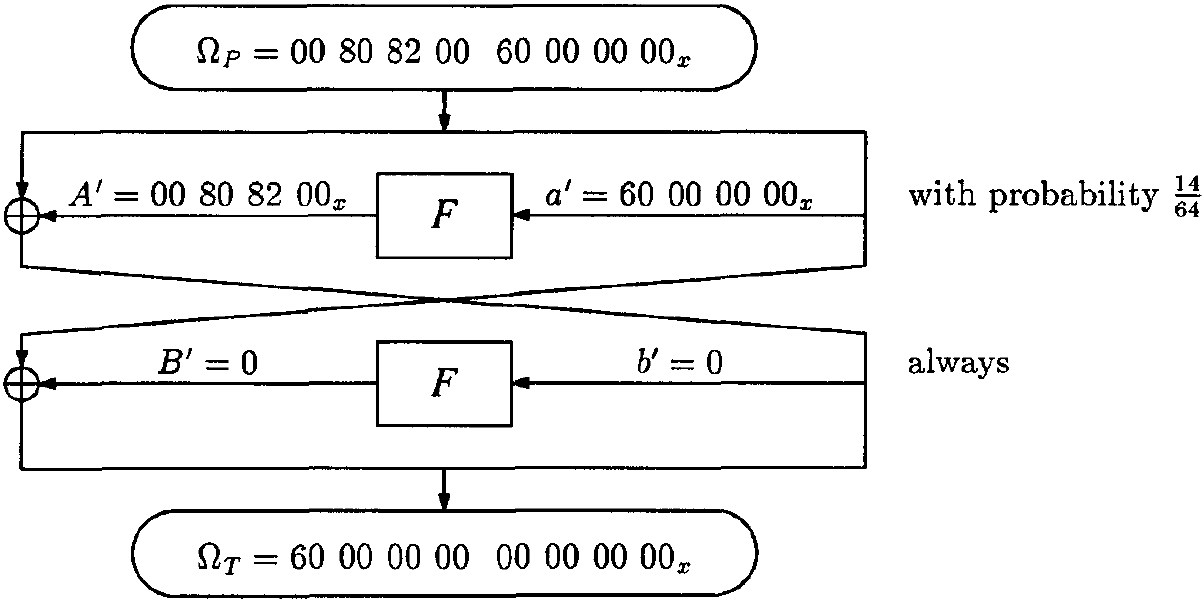
\includegraphics[width=0.9\linewidth]{images/des_char.png}
            \caption{Example of a two-round characteristic with probability \(\frac{14}{64}\).}
            \label{fig:des-char-example}
        \end{figure}
    \end{frame}

    \subsection{Signal to Noise Ratio}
    \label{subsec:snr}
    
    \begin{frame}
        \frametitle{Signal to Noise Ratio}
        \begin{enumerate}
            \item Right pairs will always suggest the right key value. But right
            pairs occur with probability \(p^\Omega\).
            \item<2-> On the other hand, wrong pairs suggest a randomly chosen
            key (not necessarily the right key in the worst case).
            \item<3-> Suitable counting approach on the key values will
            ``spike'' at the right key and have smaller but approximately equal
            counts at other keys.
            \item<4-> The key with the largest count is likely the actual key.
        \end{enumerate}
        \begin{definition}<5->[Signal-to-Noise Ratio]
            The ratio between the number of right pairs and the average count of
            incorrect subkeys in a counting scheme is called the \emph{signal to
            noise ratio of the counting scheme} and is denoted by \(S/N\).
        \end{definition}
    \end{frame}

    \begin{frame}
        \frametitle{Computing the SNR}
        Consider the variables shown in \cref{tab:snr-vars}.
        \begin{table}[!ht]
            \centering
            \begin{tabular}{|c|l|}
                \hline
                \textbf{Variable} & \textbf{Definition} \\
                \hline
                \(p\) & Probability of the characteristic \\
                \hline
                \(m\) & Number of created pairs \\
                \hline
                \(\alpha\) & Average count per analyzed pair \\
                \hline
                \(\beta\) & Fraction of analyzed pairs \\
                \hline
                \(k\) & Number of key bits counted on \\
                \hline
            \end{tabular}
            \caption{Table of variables to compute the SNR.}
            \label{tab:snr-vars}
        \end{table}
        \pause
        Then,
        \begin{equation}
            S/N = \frac{m \cdot p}{\frac{m \cdot \beta \cdot \alpha}{2^k}} = \frac{2^k \cdot p}{\alpha \cdot \beta}
            \label{eq:snr-expr}
        \end{equation}
    \end{frame}

    \subsection{Structures}
    \label{subsec:structures}

    \begin{frame}
        \frametitle{Structures}
        \begin{enumerate}
            \item<1-> Many attacks on DES use more than one characteristic.
            \item<2-> Requirement to minimize the amount of plaintexts generated.
            \begin{definition}<3->[Quartet and Octet]
                A \emph{quartet} is a structure of four ciphertexts that
                simultaneously contains two ciphertext pairs of one
                characteristic and two ciphertext pairs of a second
                characteristic. An \emph{octet} is a structure of eight
                ciphertexts that simultaneously contains four ciphertext pairs
                of each of three characteristics.
            \end{definition}
            \item<3-> As an example, \(\brak{P, P \oplus \Omega_P^1, P \oplus
            \Omega_P^2, P \oplus \Omega_P^1 \oplus \Omega_P^2}\) is a quartet.
            \item<4-> Quartets save \(\frac{1}{2}\) of the data and octets save
            \(\frac{2}{3}\) of the data.
        \end{enumerate}
    \end{frame}

    \section[Cryptanalysis]{Differential Cryptanalysis of DES Variants}
    \label{sec:cryptanalysis}

    \subsection{DES Reduced to Four Rounds}
    \label{subsec:des-4rd}

    \begin{frame}
        \frametitle{DES Reduced to Four Rounds}
        \begin{enumerate}
            \item<1-> Use two one-round characteristics, as shown in
            \cref{fig:des-4rd-char}.
            \item<2-> Both characteristics have probability 1.
            \item<3-> Example of a \emph{3R-attack}. There are \emph{three}
            extra rounds after the characteristic is applied.
        \end{enumerate}
        
        \visible<2->{
            \begin{figure}[!ht]
                \centering
                \begin{subfigure}[t]{0.4\linewidth}
                    \centering
                    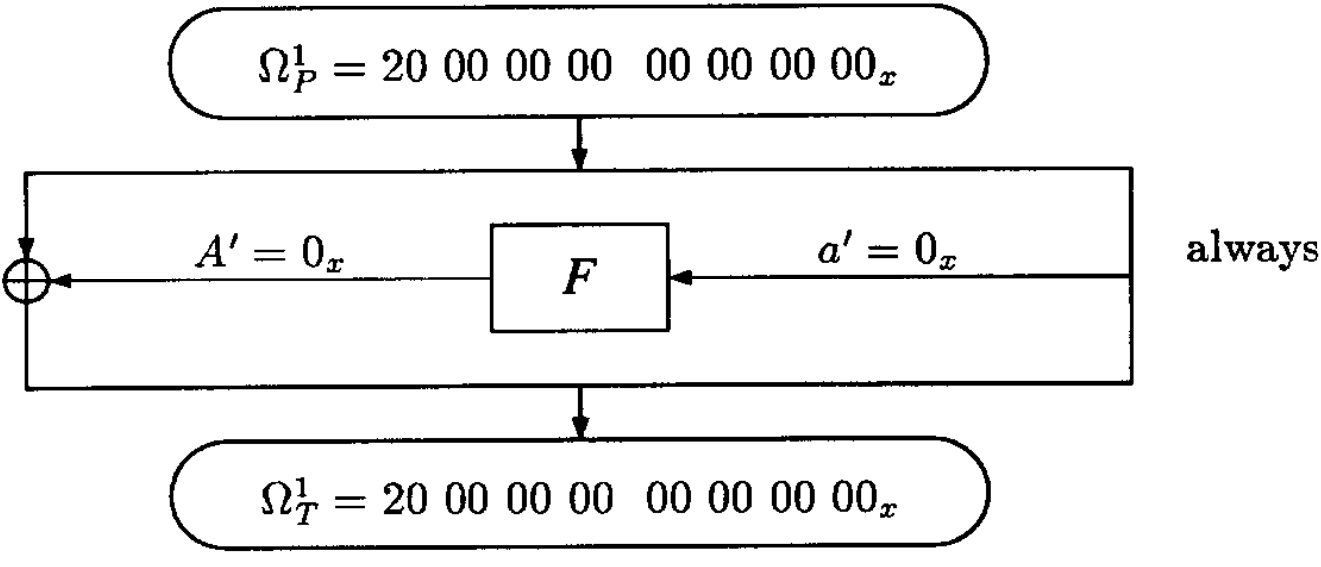
\includegraphics[width=\columnwidth]{images/des_4round_char.png}
                \end{subfigure}
                ~
                \begin{subfigure}[t]{0.4\linewidth}
                    \centering
                    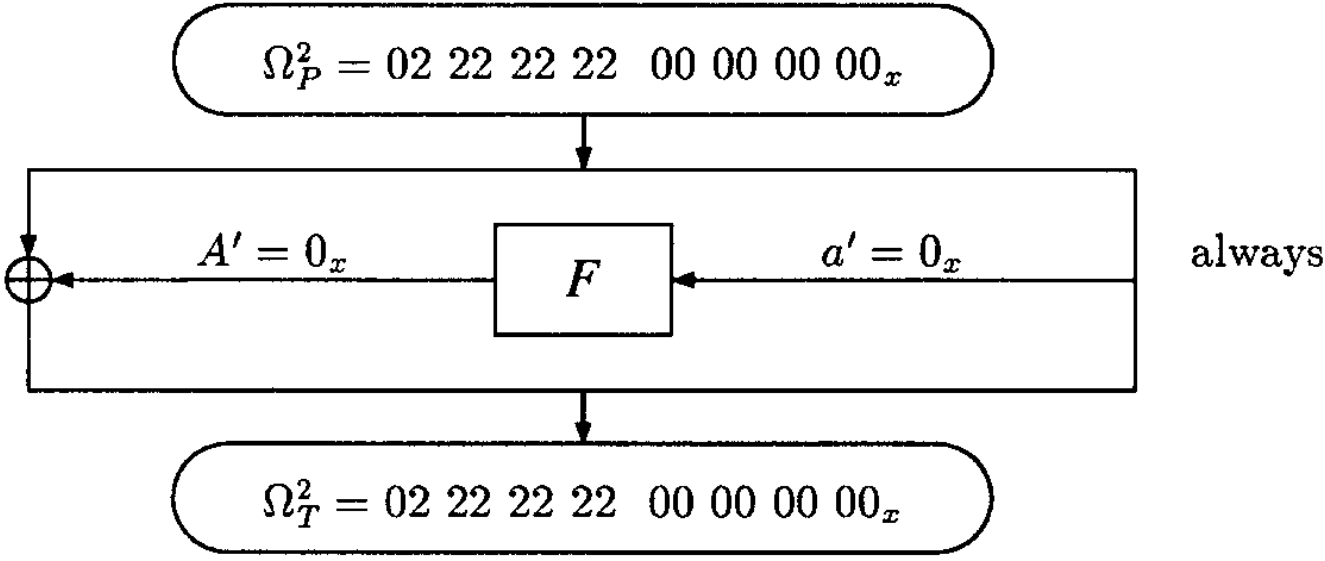
\includegraphics[width=\columnwidth]{images/des_4round_char2.png}
                \end{subfigure}
                \caption{Characteristics used for cryptanalysis of DES reduced to four rounds.}
                \label{fig:des-4rd-char}
            \end{figure}
        }
    \end{frame}

    \begin{frame}
        \frametitle{DES Reduced to Four Rounds}
        \begin{columns}
            \begin{column}{0.65\textwidth}
                \begin{enumerate}
                    \item<2-> Using \(\Omega^1\), we have
                    \begin{equation}
                        c^\prime = D^\prime \oplus l^\prime = a^\prime \oplus B^\prime \implies D^\prime = B^\prime \oplus l^\prime
                        \label{eq:des-4rd-D}
                    \end{equation}
                    \item<3-> We have \(a^\prime = 0_x \implies A^\prime = 0_x\)
                    and \(b^\prime = A^\prime \oplus L^\prime = L^\prime\).
                    \begin{itemize}
                        \item<4-> In the second round S2, \dots, S8 receive
                        zero XOR input.
                        \item<5-> 28 bits of \(B^\prime\) are zero and hence we
                        can find \emph{28 bits of \(D^\prime\)}.
                        \item<6-> We already know \(d^\prime = r^\prime\). So,
                        we employ a counting approach to get \(K4\).
                    \end{itemize}
                \end{enumerate}
            \end{column}
            \begin{column}{0.35\textwidth}
                \begin{figure}[!ht]
                    \centering
                    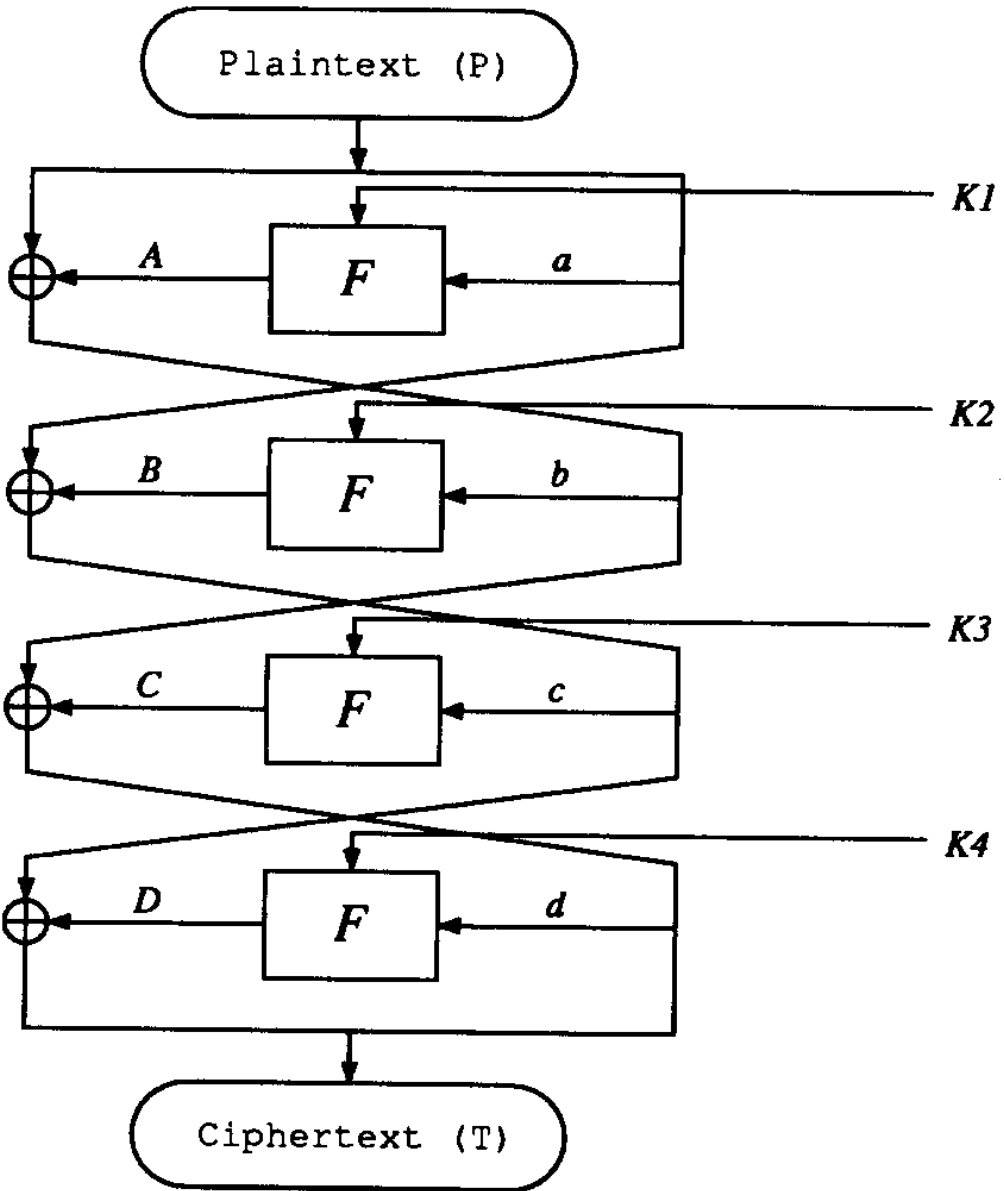
\includegraphics[width=\columnwidth]{images/des_4round.png}
                    \caption{DES reduced to four rounds.}
                    \label{fig:des-four}
                \end{figure}
            \end{column}
        \end{columns}
    \end{frame}

    \begin{frame}
        \frametitle{DES Reduced to Four Rounds}
        \begin{enumerate}
            \item<1-> To get \(Si_{Kd}\) for \(2 \le i \le 8\), we verify
            \eqref{eq:des-4rd-check}.
            \begin{equation}
                S\brak{S_{E} \oplus S_{K}} \oplus S\brak{S_{E}^* \oplus S_{K}} = S_{O}^\prime
                \label{eq:des-4rd-check}
            \end{equation}
            \item Only \emph{one} plaintext pair is needed since characteristic
            probability is 1.
            \item We recover \(7 \times 6 = 42\) key bits of \(K4\), which
            correspond to 42 bits of the master key.
            \item Exhaustively search the other 14 key bits to get the entire
            master key.
            \item We have used the key schedule to our advantage here?
            \emph{What if all the keys were independent?}
        \end{enumerate}
    \end{frame}

    \begin{frame}
        \frametitle{DES Reduced to Four Rounds: Independent Subkeys}
        \begin{enumerate}
            \item<1-> We now use \(\Omega^2\) to get the remaining 6 subkey bits
            of \(K4\), as the input to S1 in the second round is now zero.
            \item<2-> We have \(C^\prime = b^\prime \oplus d^\prime\). Peeling
            off/decrypting one round will give us \(c^\prime\) completely.
            \begin{itemize}
                \item<3-> Since \(c^\prime\) and \(C^\prime\) are both
                completely known, \(K3\) can be completely found using a similar
                counting argument.
            \end{itemize}
            \item<4-> Since \(a^\prime = A^\prime = 0_x\), all keys are equally
            likely. Other characteristics \(\Omega^3\) and \(\Omega^4\) are
            chosen such that
            \begin{itemize}
                \item \(S_{Ea}^\prime \neq 0_x\) for all S boxes for both
                characteristics.
                \item For every S box, the \(S_{Ea}^\prime\) values differ
                between the characteristics.
                \item Similar counting methods used to get \(K1\) and \(K2\).
            \end{itemize}
            \item<5-> 16 chosen plaintexts are needed for this attack.
            \begin{itemize}
                \item 8 pairs of \(\Omega^1\) and \(\Omega^2\) each.
                \item 4 pairs of \(\Omega^3\) and \(\Omega^4\) each.
            \end{itemize}
            To reduce the data needed, two octets are used.
        \end{enumerate}
    \end{frame}

    \subsection{DES Reduced to Six Rounds}
    \label{subsec:des-6rd}

    \begin{frame}
        \frametitle{DES Reduced to Six Rounds}
        \begin{enumerate}
            \item Two three-round characteristics used, each with probability
            \(\frac{1}{16}\).
            \item<2-> We have,
            \begin{equation}
                e^\prime = c^\prime \oplus D^\prime = F^\prime \oplus l^\prime \implies F^\prime = c^\prime \oplus D^\prime \oplus l^\prime
            \end{equation}
        \end{enumerate}
        \begin{figure}[!ht]
            \centering
            \begin{subfigure}{0.4\linewidth}
                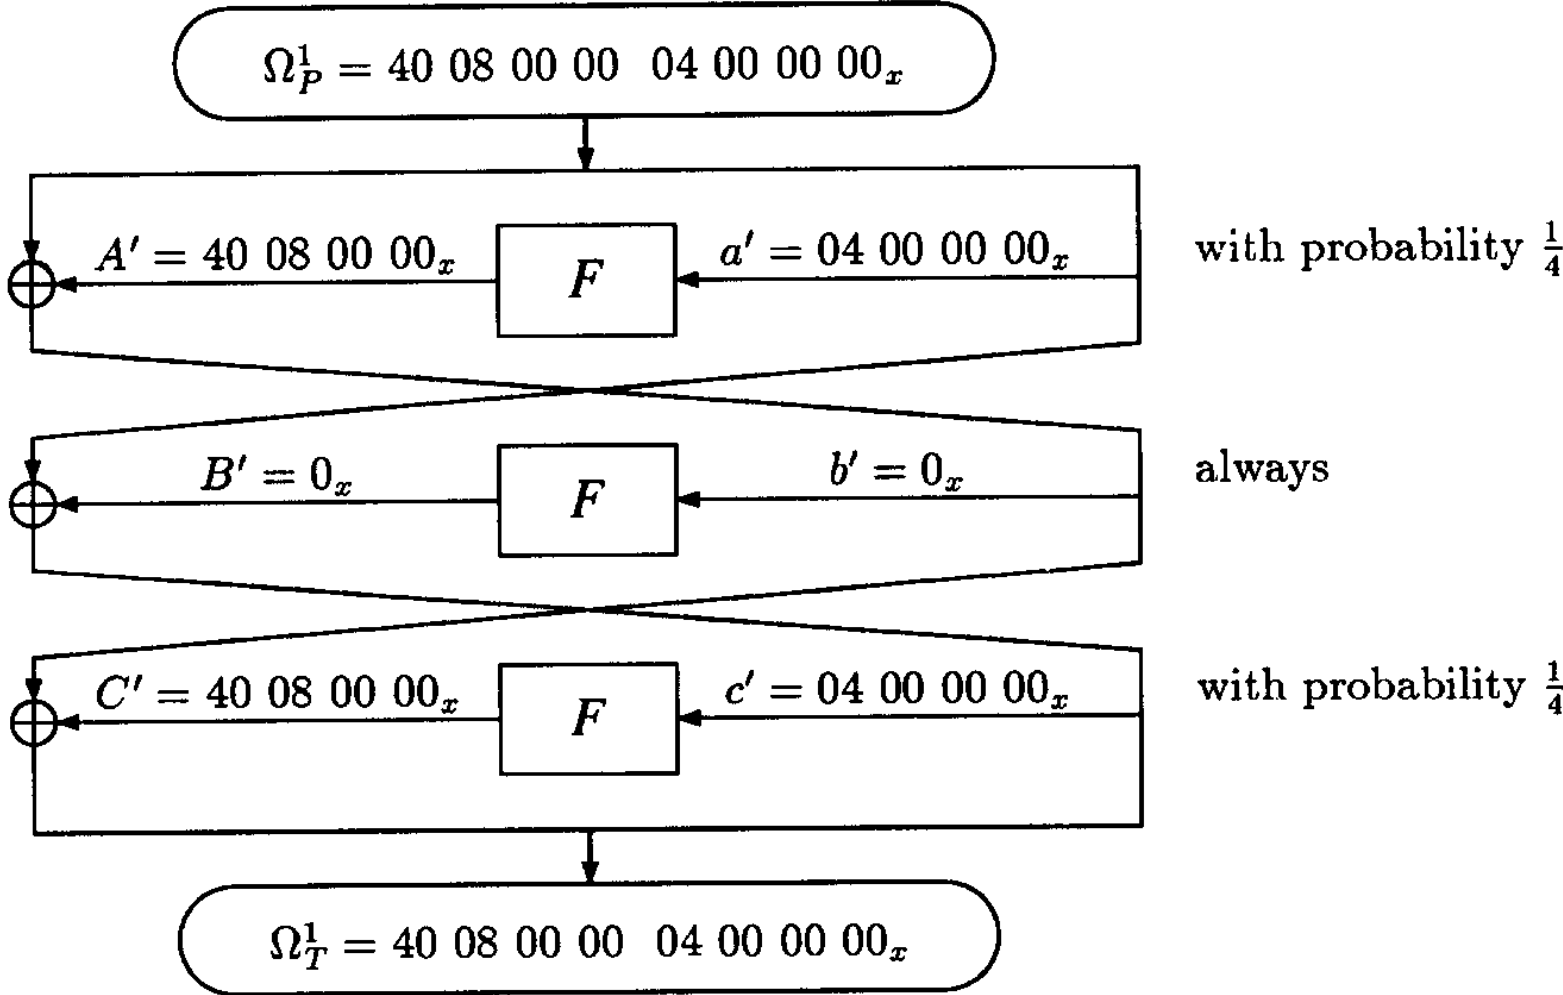
\includegraphics[width=\columnwidth]{images/des_6round_char1.png}
            \end{subfigure}
            ~
            \begin{subfigure}{0.4\linewidth}
                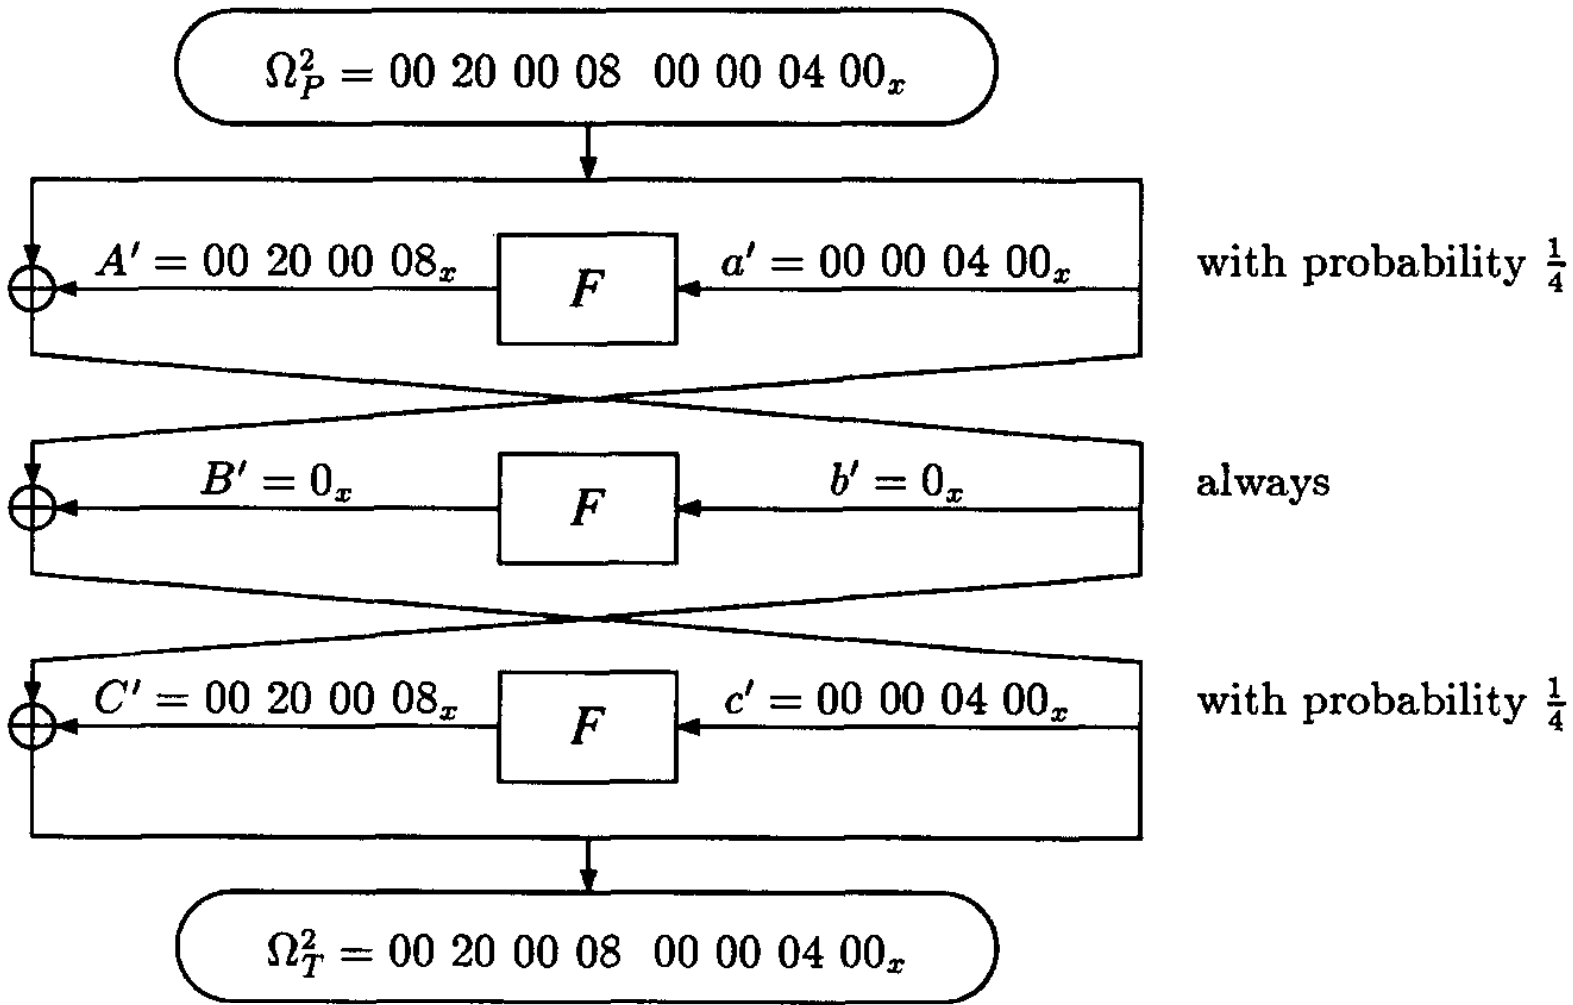
\includegraphics[width=\columnwidth]{images/des_6round_char2.png}
            \end{subfigure}
            \caption{Characteristics used for cryptanalysis of DES reduced to 6 rounds.}
            \label{fig:des-6-char}
        \end{figure}
    \end{frame}

    \begin{frame}
        \frametitle{DES Reduced to Six Rounds}
        \begin{enumerate}
            \item<1-> In the fourth round,
            \begin{itemize}
                \item with \(\Omega^1\), S2, S5, \dots, S8 have zero input XORs.
                \item with \(\Omega^2\), S1, S2, S4, S5 and S6 have zero input
                XORs.
            \end{itemize}
            \item<2-> Combining both characteristics, 42 key bits of \(K6\) can
            be found.
            \item<3-> Counting on more bits gives high \(S/N\) at the cost of
            exponentially more memory.
            \item<4-> Due to higher \(S/N\), fewer plaintext pairs are analyzed.
            \emph{This is exploited to get a faster counting algorithm}.
        \end{enumerate}
    \end{frame}

    \begin{frame}
        \frametitle{The Clique Method}
        \begin{enumerate}
            \item<1-> Used to reduce memory when few plaintexts are used to
            count on more subkey bits.
            \item<2-> Create a graph where
            \begin{itemize}
                \item Each plaintext pair is a vertex.
                \item There is an edge between two vertices if corresponding
                pairs suggest the same key value for an S box.
            \end{itemize}
            \item<3-> The edges are labelled with five 64-bit masks (one mask
            per S box, one bit per suggested key value in the mask).
            \begin{itemize}
                \item A pair suggests a key value if it passes the check in
                \eqref{eq:des-4rd-check}.
            \end{itemize}
            \item<4-> Goal is to find the largest clique such that the bitwise
            AND of all masks in the subgraph induced by that clique is nonzero.
            \item<5-> Apply this method for both \(\Omega^1\) and \(\Omega^2\),
            ensuring that the suggested keys at S2, S5 and S6 match. Otherwise,
            use more data.
        \end{enumerate}
    \end{frame}

    \begin{frame}
        \frametitle{Completing the Cryptanalysis}
        \begin{columns}
            \begin{column}{0.6\linewidth}
                \begin{enumerate}
                    \item<1-> 42 key bits have been found, can exhaustively
                    search remanining 14 bits.
                    \item<2-> Speed up the search by finding remaining 6 key
                    bits of \(K6\) using \cref{fig:des-k5}. Count using checks
                    on S2, S3 and S8 of the fifth round. 
                    \begin{itemize}
                        \item<3-> Exhaustively search remaining 8 bits.
                        \item<4-> Discard wrong pairs by checking if they
                        satisfy the characteristic and expected value of
                        \(F^\prime\).
                        \item<5-> Leaves \(\frac{1}{16}\) of the pairs, boosts
                        \(S/N\).
                    \end{itemize}
                \end{enumerate}
            \end{column}
            \begin{column}{0.4\linewidth}
                \begin{figure}[!ht]
                    \centering
                    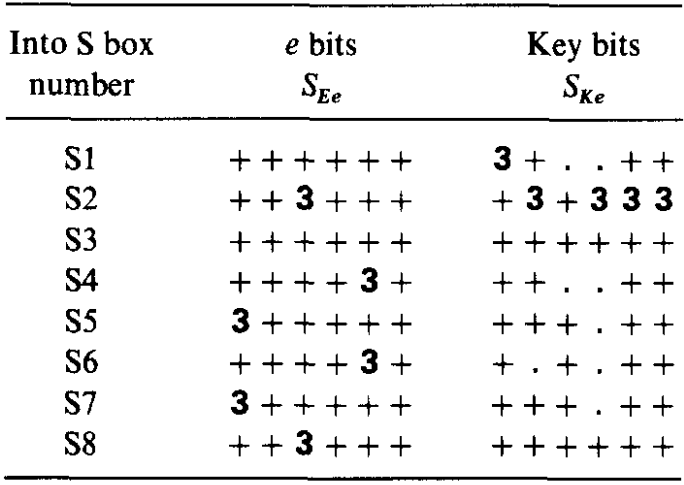
\includegraphics[width=\columnwidth]{images/des_k5.png}
                    \caption{Dependence of \(K5\) on \(K6\). `3' indicates
                    dependence on \(S3_{Kf}\), `.' indicates bits unused in K6
                    and `+' indicates dependence on known key bits of K6.}
                    \label{fig:des-k5}
                \end{figure}
            \end{column}
        \end{columns}
    \end{frame}

    \begin{frame}
        \frametitle{Data Requirements}
        \begin{enumerate}
            \item<1-> The first phase has
            \begin{equation}
                S/N = \frac{2^{30} \cdot \frac{1}{16}}{4^5} = 2^{16}.
            \end{equation}
            Only 7-8 pairs are needed for each characteristic. Since each
            characteristic has probability \(\frac{1}{16}\), we require about
            120 pairs of plaintexts.
            \item<2-> The second phase has
            \begin{equation}
                S/N = \frac{2^6 \cdot 1}{4} = 16.
            \end{equation}
            Though \(S/N\) is lesser, we can use the 7-8 right pairs from the
            first part.
            \item<3-> We can reduce the data required by using quartets. In
            total, about 240 ciphertexts are needed. 
        \end{enumerate}
    \end{frame}

    \subsection{DES Reduced to Eight Rounds}
    \label{subsec:des-8rd}

    \begin{frame}
        \frametitle{DES Reduced to Eight Rounds}
        \begin{columns}
            \begin{column}{0.6\linewidth}
                \begin{enumerate}
                    \item We use a 5-round characteristic with probability
                    \(\approx \frac{1}{10486}\).
                    \item From \cref{fig:des-8rd-char}, a right pair has
                    \(f^\prime = d^\prime \oplus E^\prime = 40\ 5C\ 00\ 00_x\).
                    \begin{itemize}
                        \item In the sixth round, S2, S5, \dots, S8 have zero
                        input XORs.
                    \end{itemize}
                    \item We have,
                    \begin{align}
                        g^\prime = e^\prime \oplus F^\prime &= H^\prime \oplus l^\prime \\
                        \implies H^\prime &= e^\prime \oplus F^\prime \oplus l^\prime.
                    \end{align}
                \end{enumerate}
            \end{column}
            \begin{column}{0.4\linewidth}
                \begin{figure}[!ht]
                    \centering
                    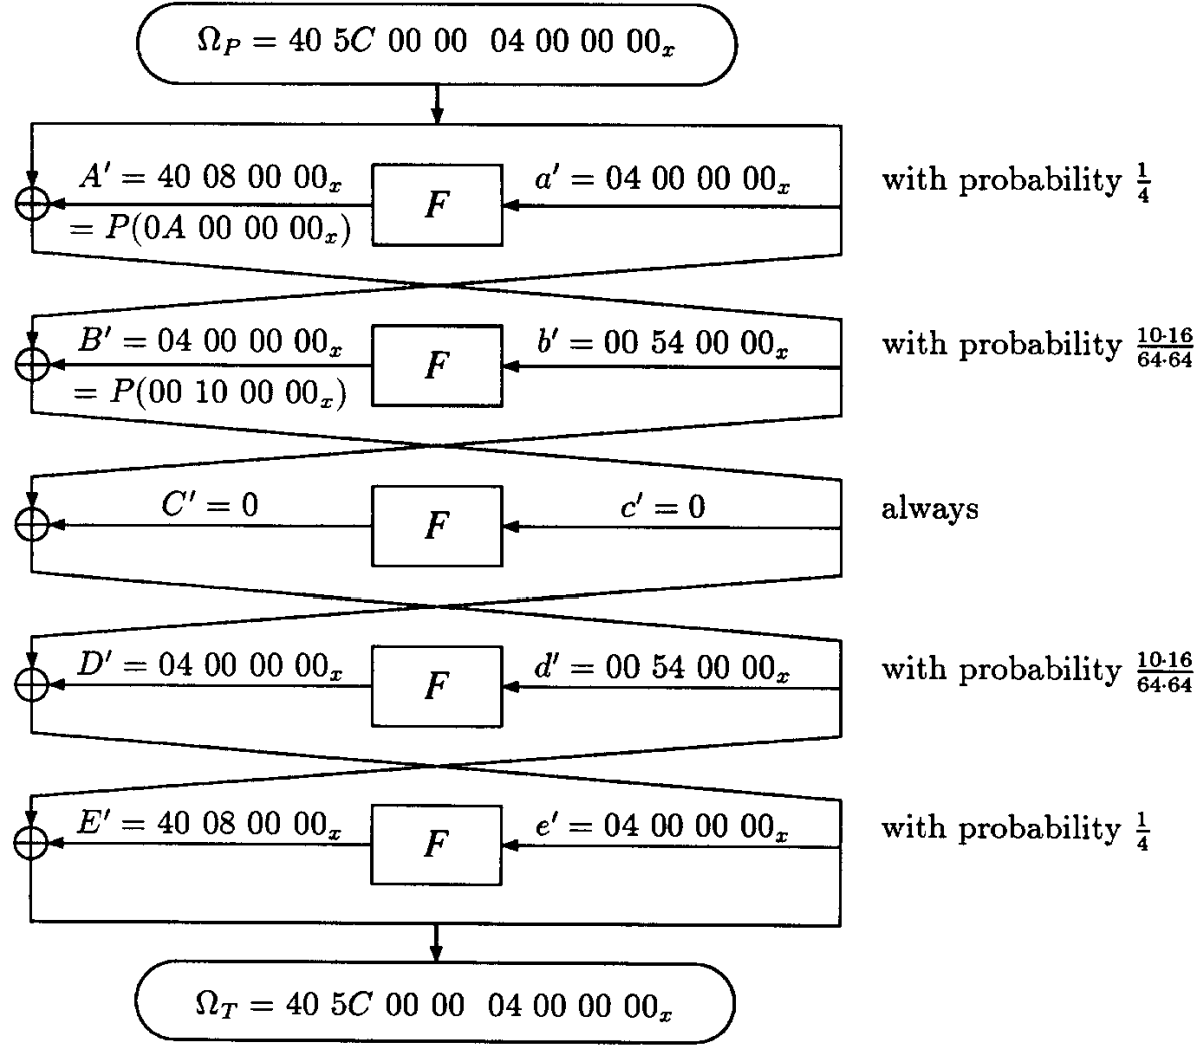
\includegraphics[width=\columnwidth]{images/des_8round_char.png}
                    \caption{5 round characteristic to cryptanalyze DES reduced to 8 rounds.}
                    \label{fig:des-8rd-char}
                \end{figure}
            \end{column}
        \end{columns}
    \end{frame}

    \begin{frame}
        \frametitle{Improving the Signal to Noise Ratio}
        \begin{enumerate}
            \item<1-> Signal to noise ratio for
            \begin{itemize}
                \item \(k = 30\) is \(S/N = \frac{2^{30}}{4^5 \cdot 10486}
                \approx 100\). Requires \(2^{30}\) counters.
                \item \(k = 24\) is \(S/N = \frac{2^{24}}{4^4 \cdot 0.8 \cdot
                10486} \approx 7.8\). Requires \(2^{24}\) counters.
                \item \(k = 18\) is \(S/N = \frac{2^{18}}{4^3 \cdot 0.8^2 \cdot
                10486} \approx 0.6\). Requires \(2^{18}\) counters.
            \end{itemize}
            \only<2->{\emph{Why the 0.8 in the denominator?}}
            \item<3-> If counting on fewer S boxes, choose the ones that
            \emph{maximize} the characteristic probability, and check against
            the other S boxes.
            \item<4-> Notice that
            \begin{equation}
                e^\prime = 04\ 00\ 00\ 00_x \rightarrow E^\prime = P\brak{0W\ 00\ 00\ 00_x} = X0\ 0Y\ Z0\ 00_x
                \label{eq:des-8rd-e-E}
            \end{equation}
            where \(W \in \cbrak{0,1,2,3,8,9,A,B},\ X,Z \in \cbrak{0,4},\ Y \in
            \cbrak{0,8}\).
            \item<5-> Thus, \(f^\prime = d^\prime \oplus E^\prime = X0\ 5V\ Z0\
            00_x\) where \(V = Y \oplus 4\).
            \begin{itemize}
                \item \(Z = 0 \implies E^\prime = 40\ 08\ 00\ 00_x\). This
                happens with probability \(\frac{16}{64}\).
                \item All other possiblities having \(Z = 4\) happen with
                probability \(\frac{20}{64}\).
            \end{itemize}
        \end{enumerate}
    \end{frame}

    \begin{frame}
        \frametitle{Modifying the Characteristic}
        \begin{enumerate}
            \item<1-> From \eqref{eq:des-8rd-e-E}, the modified probability of
            \(e^\prime \rightarrow E^\prime\) is \(\frac{16}{64} +
            0.8\frac{20}{64} = \frac{1}{2}\).
            \item<2-> \emph{We have doubled the characteristic probability to
            \(\frac{1}{5243}\)}! Thus, for \(k = 24, S/N \approx 15.6\) and for
            \(k = 18, S/N \approx 1.2\).
            \begin{itemize}
                \item<3-> Key bits of S5 NOT counted, but used for checking as
                in \eqref{eq:des-4rd-check}.
            \end{itemize}
            \item<4-> For \(k = 24\), we need \(25000\) pairs. For \(k = 18\),
            we need \(150000\) pairs, where
            \begin{itemize}
                \item Average count per key is \(\frac{150000 \cdot 4^3 \cdot
                0.8^2}{2^{18}} = 24\).
                \item Right key is counted an additional \(\frac{150000}{5243} =
                29\) times, for a total count of \(24 + 29 = 53\).
            \end{itemize}
            \item<5-> After counting on 18 key bits, we count on S2 and S5 of the
            last round using the 53 filtered pairs.
            \begin{itemize}
                \item Almost all remanining pairs after both counting schemes
                should be right pairs (why?).
                \item<6-> \emph{Hint: What is the probability that a wrong pair
                survives both counting stages?}
            \end{itemize}
        \end{enumerate}
    \end{frame}

    \begin{frame}
        \frametitle{Finding the Remaining Bits of \(K8\)}
        \begin{columns}
            \begin{column}{0.6\linewidth}
                \begin{enumerate}
                    \item<1-> Since 20 bits of \(H\) and \(H^*\) are known we
                    can get corresponding bits of \(g\) and \(g^*\). 
                    \item<2-> Exhaustive search performed for the remaining 18
                    bits of \(K8\). We know \(G^\prime = f^\prime \oplus
                    h^\prime\).
                    \begin{itemize}
                        \item Search for the 12 bits entering S1 and S4 by
                        verifying \(S3_{Og}^\prime\).
                        \item Then exhaustively search for the other 6 bits
                        using the relations in \cref{fig:des-8rd-dep}.
                    \end{itemize}
                    \item<3-> The last 8 bits can also be exhaustively searched
                    using one ciphertext pair.
                \end{enumerate}
            \end{column}
            \begin{column}{0.4\linewidth}
                \visible<2->{
                    \begin{figure}[!ht]
                        \centering
                        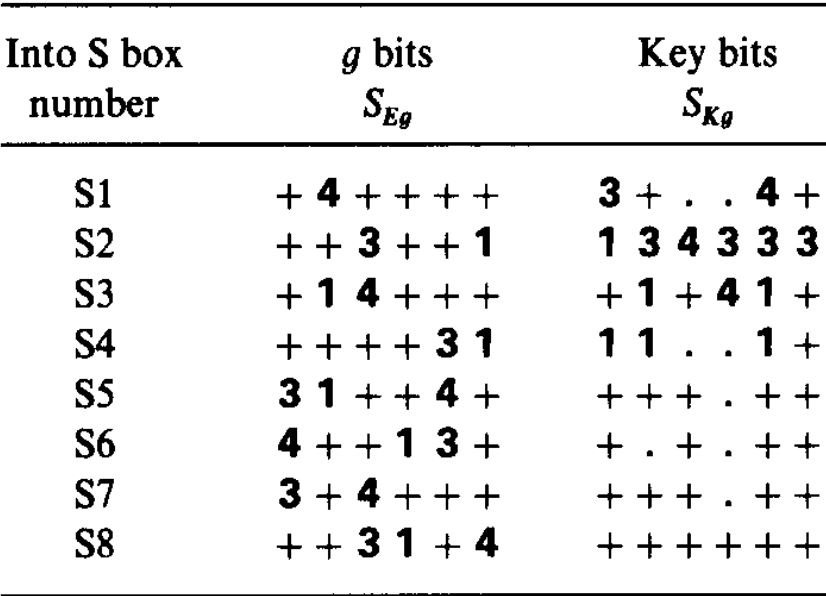
\includegraphics[width=\columnwidth]{images/des_8round_dep.png}
                        \caption{Dependence of \(K7\) on \(K8\).}
                        \label{fig:des-8rd-dep}
                    \end{figure}
                }
            \end{column}
        \end{columns}
    \end{frame}

    \begin{frame}
        \frametitle{Memory Saving Techniques}
        \begin{enumerate}
            \item<1-> We can discard wrong pairs as and when they are
            identified. Leaves \(0.8^5 \approx \frac{1}{3}\) of all pairs.
            \begin{itemize}
                \item<2-> Still not enough for 18 bits (reduces to 50000 pairs).
            \end{itemize} 
            \item<3-> Use a \emph{heuristic} weighting function to discard even
            more wrong pairs.
            \begin{itemize}
                \item<4-> Based on the idea that a right pair suggests more key
                values than a wrong pair.
                \item<5-> Weighting function is product of key values suggested
                by the five countable S boxes of the last round.
                \item<6-> Threshold chosen to discard most wrong pairs.
                Experimentally good threshold is 8192 which discards 97\% of the
                wrong pairs.
            \end{itemize}
            \item<7-> The weighting function reduces number of analyzed pairs to
            7500, leading to improvements in runtime.
        \end{enumerate}
    \end{frame}

    \begin{frame}
        \frametitle{Enhanced Characteristic's Probability}
        \begin{enumerate}
            \item<1-> Use relations between input and output bits of the S boxes
            in the characteristic to refine choices for plaintexts.
            \item<2-> Main idea:
            \begin{itemize}
                \item Find relation between input bits for a high probability
                entry in the pairs XOR distribution table.
                \item Find information about the key bits at those positions
                (this could be found earlier).
                \item Choose plaintexts accordingly to boost characteristic
                probability and signal to noise ratio.
            \end{itemize}
        \end{enumerate}
    \end{frame}

    \begin{frame}
        \frametitle{Extension to Nine Rounds}
        \begin{columns}
            \begin{column}{0.6\linewidth}
                \begin{enumerate}
                    \item<1-> Characteristic shown in \cref{fig:des-8rd-char}
                    extended with extra round shown in \cref{fig:des-9rd-char}.
                    \item<2-> Characteristic probability \(\approx 10^{-6}\).
                    \begin{itemize}
                        \item \(S/N = \frac{2^{30}}{4^5 \cdot 10^6} \approx 1\).
                        \item About 30 million pairs and an array of \(2^{30}\)
                        counters needed.
                    \end{itemize}
                    \item<3-> This attack requires a lot of data and memory,
                    hence it is unrealistic.
                \end{enumerate} 
            \end{column}
            \begin{column}{0.4\linewidth}
                \begin{figure}[!ht]
                    \centering
                    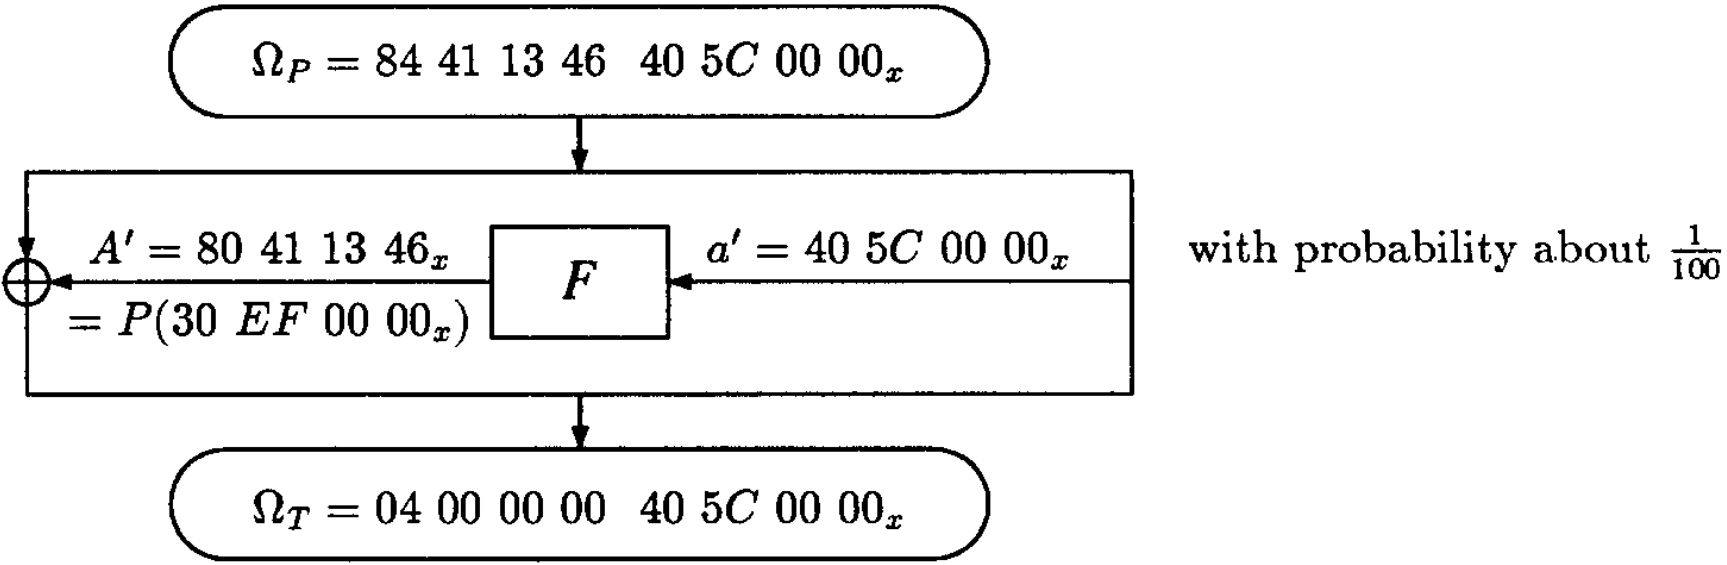
\includegraphics[width=\columnwidth]{images/des_9round_char.png}
                    \caption{Extension of characteristic for cryptanalysis of DES reduced to 9 rounds.}
                    \label{fig:des-9rd-char}
                \end{figure}
            \end{column}
        \end{columns}
    \end{frame}

    \subsection{DES with an Arbitrary Number of Rounds}
    \label{subsec:des-arbit}

    \begin{frame}
        \frametitle{Iterative Characteristics}
        \begin{columns}
            \begin{column}{0.6\linewidth}
                \begin{enumerate}
                    \item<1-> Can concatenate with itself to create longer
                    characteristics. Useful for arbitrary rounds.
                    \item<2-> \cref{fig:des-iter-char} shows a characteristic
                    with optimal probability (why?).
                    \begin{itemize}
                        \item<3-> Another value of \(\psi = 1B\ 60\ 00\ 00_x\).
                    \end{itemize}
                    \item<4-> Add an extra round for ``free'' by concatenating
                    just the first round again.
                    \item<5-> 15-round extension has probability \(2^{-56}\).
                    \emph{Just the iterative characteristic is not enough}!
                \end{enumerate}
            \end{column}
            \begin{column}{0.4\linewidth}
                \begin{figure}[!ht]
                    \centering
                    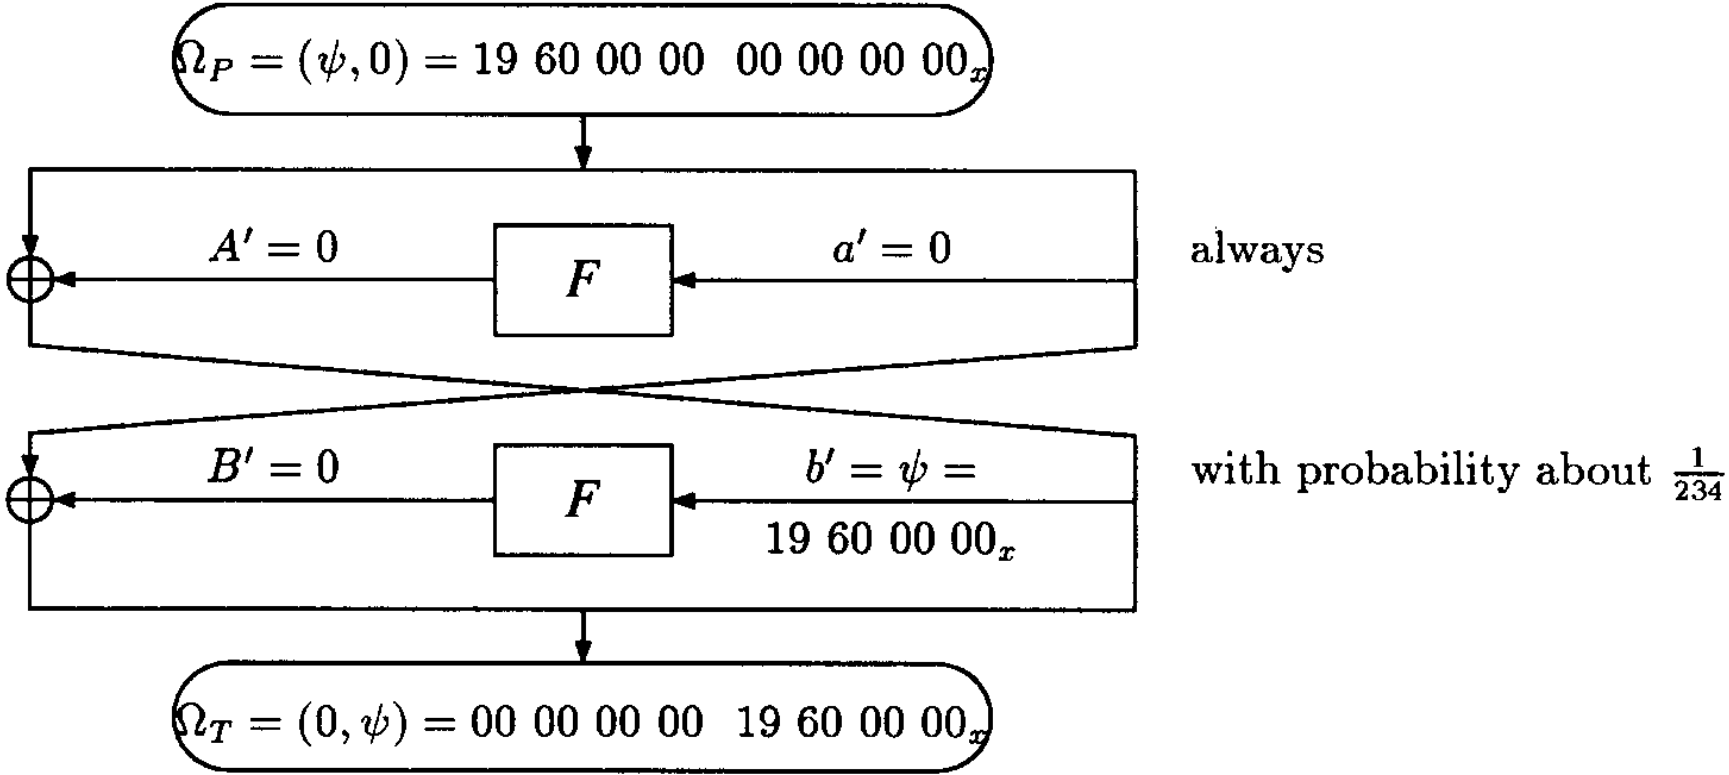
\includegraphics[width=\columnwidth]{images/des_iter_char.png}
                    \caption{An iterative characteristic for DES.}
                    \label{fig:des-iter-char}
                \end{figure}
            \end{column}
        \end{columns}
    \end{frame}

    \begin{frame}
        \frametitle{3R-Attacks}
        \begin{enumerate}
            \item<1-> Counting done on subkey bits of the last round that enter
            S boxes whose corresponding S boxes in the round which follows the
            last round of the characteristic have zero input XORs.
            \begin{itemize}
                \item<2-> In DES reduced to \emph{four} rounds: ``\dots zero
                input XORs in\dots the \emph{second} round''.
            \end{itemize}
            \item<3-> Not advisable for larger rounds due to small \(S/N\).
            \item<4-> More powerful compared to 0R/1R/2R-attacks due to smaller
            characteristic length.
            \begin{itemize}
                \item For fixed number of iterations in a cryptosystem,
                3R-attacks are the most useful.
            \end{itemize}
        \end{enumerate}
    \end{frame}

    \begin{frame}
        \frametitle{2R-Attacks}
        \begin{enumerate}
            \item<1-> Count on all bits of the subkey of the last round (why?).
            \item<2-> Wrong pairs discarded if input XORs of S boxes in the
            previous round may not cause expected output XORs.
            \item<3-> Example: DES reduced to 9 rounds.
            \begin{itemize}
                \item<3-> 7-round iterative characteristic has probability
                \(\approx 2^{-24}\).
                \item<4-> Five S boxes in the eighth round have \(S_{Eh}^\prime
                = S_{Ih}^\prime = 0\), thus \(S_{Oh}^\prime = 0\). This happens
                for wrong pairs with probability \(\frac{1}{16}\). For other S
                boxes, this probability is \(0.8\).
                \item<5-> Counting on 48 bits of \(K9\) has \(S/N = \frac{2^{48}
                \cdot 2^{-24}}{4^8 \cdot 0.8^3 \cdot \brak{\frac{1}{16}}^5}
                \approx 2^{29}\).
                \item<6-> Counting on 18 bits of \(K9\) has \(S/N = \frac{2^{18}
                \cdot 2^{-24}}{4^3 \cdot 0.8^5 \cdot 0.8^3 \cdot
                \brak{\frac{1}{16}}^5} \approx 2^{11}\).
                \item<7-> Total of \(2^{26}\) pairs needed. Filtering on last
                two rounds leaves \(0.8^3 \cdot \brak{\frac{1}{16}}^5 \cdot
                0.8^8 \approx 2^{-24}\) of wrong pairs. \emph{The clique method
                can be used since there are few pairs}.
            \end{itemize}
        \end{enumerate}
    \end{frame}

    \begin{frame}
        \frametitle{1R-Attacks}
        \begin{enumerate}
            \item<1-> Count on all bits of the subkey of the last round entering
            the S boxes with nonzero input XORs.
            \item<2-> Verify against \(r^\prime\) itself and perform possibility
            checks on other S boxes in the last round.
            \item<3-> Example: DES reduced to 10 rounds.
            \begin{itemize}
                \item<3-> 9-round iterative characteristic has probability
                \(\approx 2^{-32}\).
                \item<4-> Right pairs have \(r^\prime = \psi\) and 20 btits in
                \(l^\prime\) going out of S4, \dots, S8 are zero.
                \item<5-> Wrong pairs pass these checks with probability
                \(2^{-52}\). Thus, counting on 18 key bits has \(S/N =
                \frac{2^{18} \cdot 2^{-32}}{4^3 \cdot 2^{-52}} = 2^32\).
                \(2^{34}\) pairs are needed.
            \end{itemize}
        \end{enumerate}
    \end{frame}

    \section[Cryptanalysis of Full DES]{Differential Cryptanalysis of the Full DES}
    \label{sec:dc-des-full}

    \subsection{Summary of Differential Cryptanalysis}
    \label{subsec:dc-summary}

    \begin{frame}
        \frametitle{Complexity of Differential Cryptanalysis Attacks So Far}
        \begin{figure}[!ht]
            \centering
            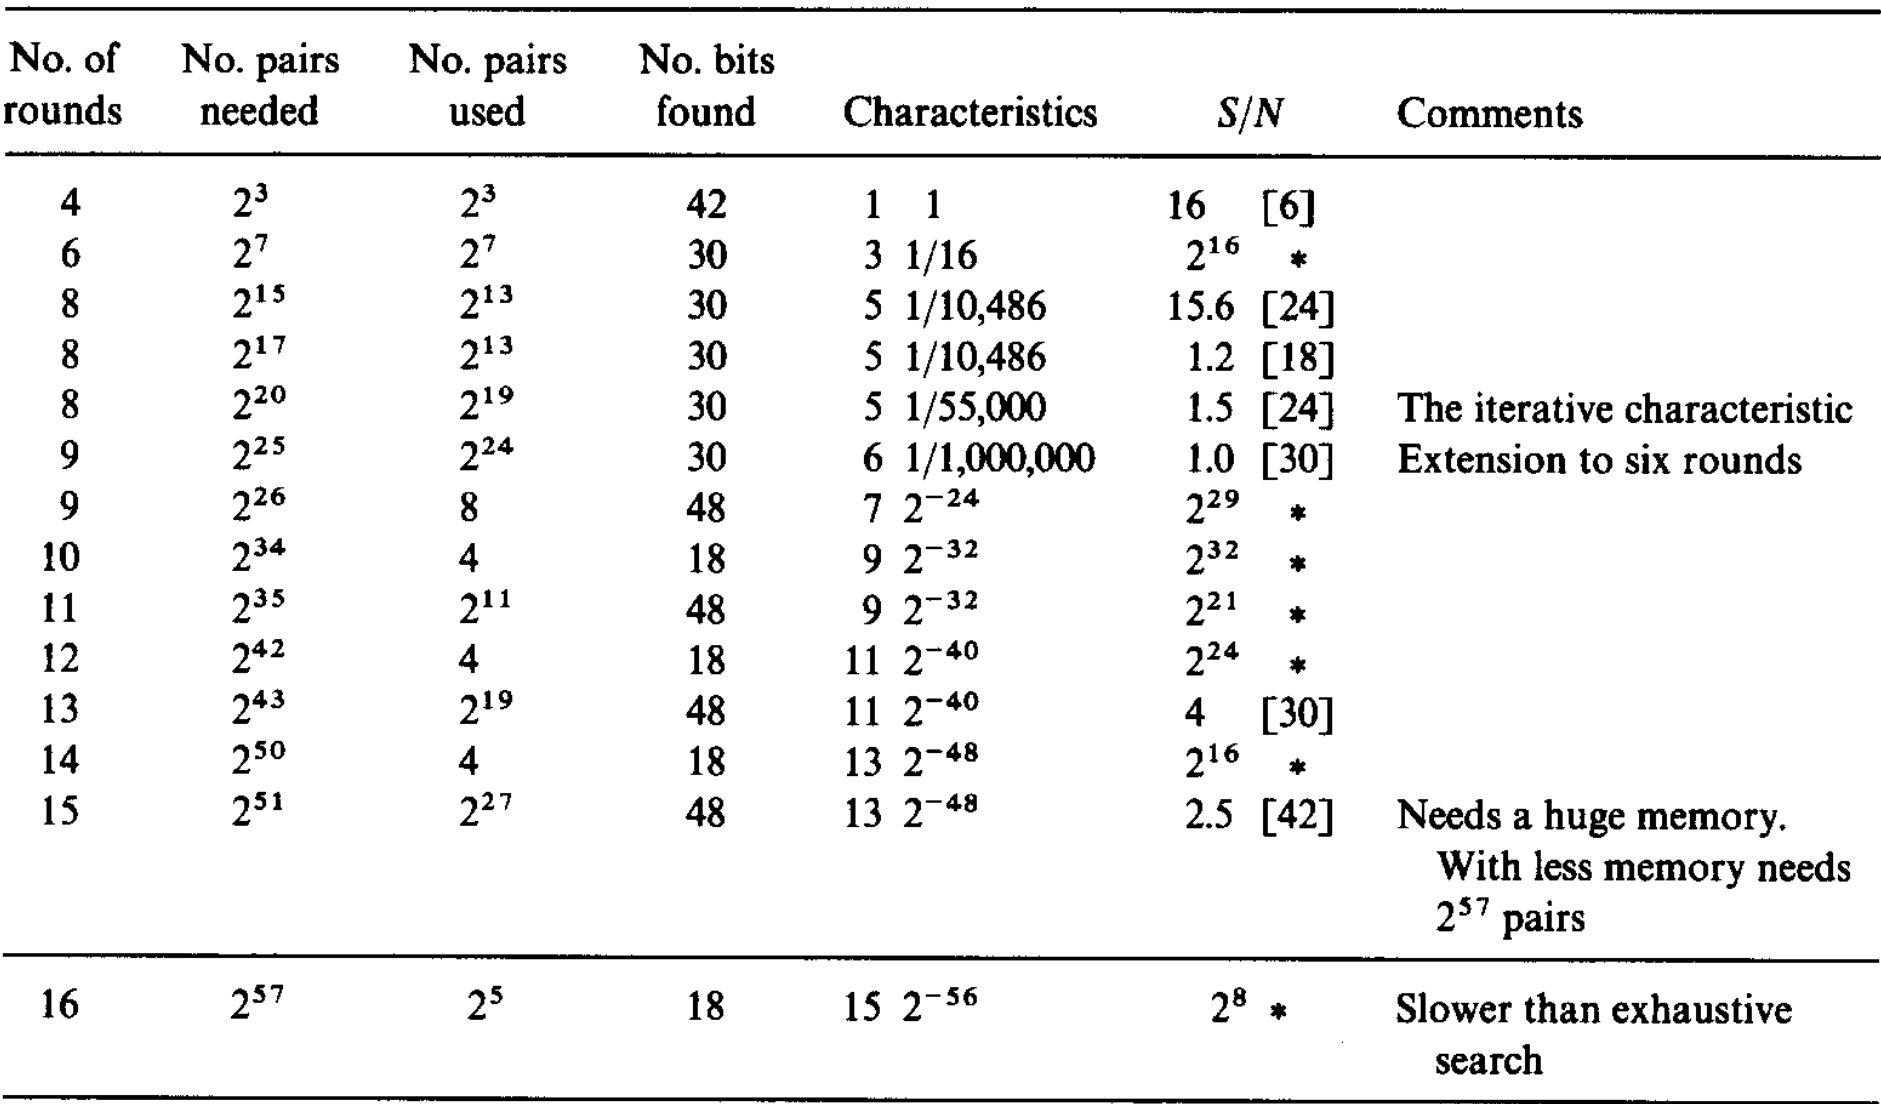
\includegraphics[width=0.7\linewidth]{images/summary.png}
            \caption{Summary of time and space complexity of differential cryptanalysis on DES.}
            \label{fig:des-summary}
        \end{figure}
    \end{frame}

    \begin{frame}
        \frametitle{Main Idea of the New Attack}
        \begin{enumerate}
            \item<1-> The iterative characteristic by itself is not enough due
            to low probability.
            \item<2-> We need to add an \emph{extra} round at no additional
            cost.
            \item<3-> A new round 1 created followed by 15-round 2R-attack to
            speed up cryptanalysis and reduce memory.
            \item<4-> This attack has two phases: \emph{data collection} and
            \emph{data analysis}.
        \end{enumerate}
    \end{frame}

    \subsection{Data Collection Phase}
    \label{subsec:data-collection}

    \begin{frame}
        \frametitle{Data Collection Phase}
        \begin{columns}
            \begin{column}{0.5\linewidth}
                \begin{enumerate}
                    \item<1-> Want to generate plaintexts that are fed to
                    15-round attack after first round.
                    \item<2-> Let \(v_0, \ldots, v_{4095}\) be the \(2^{12}\)
                    32-bit constants consisting of all possible values at the 12
                    output positions of S1, S2 and S3 after the first round, and
                    zero elsewhere.
                \end{enumerate}
            \end{column} 
            \begin{column}{0.5\linewidth}
                \begin{figure}[!ht]
                    \centering
                    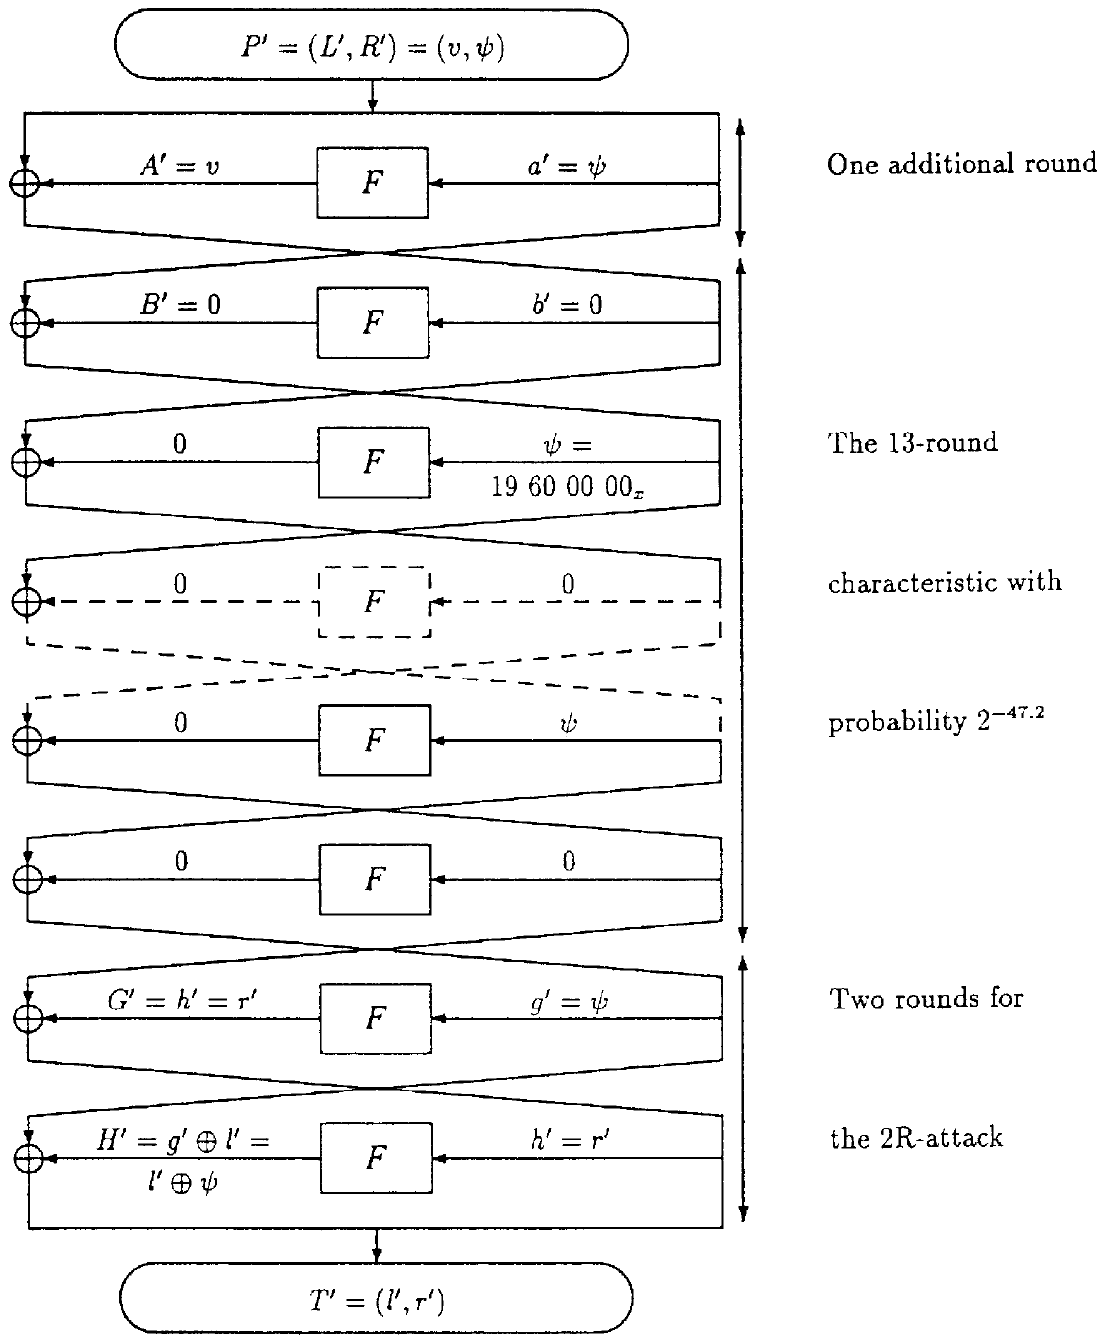
\includegraphics[height=0.65\textheight]{images/des_new_attack.png}
                    \caption{Modified 2R-attack on DES.}
                    \label{fig:des-new}
                \end{figure}
            \end{column}
        \end{columns}
    \end{frame}

    \begin{frame}
        \frametitle{Data Collection Phase}
        \begin{enumerate}
            \item<1-> For arbitrary 64-bit \(P\), define
            \begin{align}
                P_i &\triangleq P \oplus \brak{v_i, 0} \\
                \bar{P_i} &\triangleq \brak{P \oplus \brak{v_i, 0}} \oplus \brak{0, \psi} \\
                T_i &\triangleq DES\brak{P_i, K} \\
                \bar{T_i} &\triangleq DES\brak{\bar{P_i}, K}.
                \label{eq:pi-ti-def}
            \end{align}
            \item<2-> Observe that \(P_i \oplus \bar{P_j} = \brak{v_k, \psi}\).
            Each \(v_k\) occurs exactly \(2^{12}\) times (why?).
            \item<3-> \emph{We still don't know the best \(k\) for which \(\psi
            \rightarrow v_k\)}.
            \begin{itemize}
                \item<4-> Exhaustive search over the \(2^{24}\) pairs is too
                slow.
                \item<5-> Exploit the cross-product structure to speed up the
                search.
            \end{itemize}
        \end{enumerate}
    \end{frame}

    \begin{frame}
        \frametitle{Data Collection Phase}
        \begin{enumerate}
            \item<1-> A right pair has zero output XOR at S4, \dots, S8 of the
            last round.
            \item<2-> Hash the \(2^{13}\) plaintexts \(P_i, \bar{P_i}\) based on
            these \(2^{20}\) values. Only \(2^{24} \cdot 2^{-20} = 2^4 = 16\)
            pairs will survive.
            \item<3-> Additional S boxes can be tested in the first, fifteenth
            and sixteenth ronud to discard about 92.55\% of surviving pairs,
            leaving about \(16 \cdot 0.0745 = 1.19\) pairs per structure.
            \begin{itemize}
                \item<4-> Input XOR for right pairs in first and fifteenth
                rounds are fixed, so use number of non-zero entries of
                corresponding lines in the pairs XOR distribution table.
                Fraction of surviving pairs is \(\brak{\frac{14}{16} \cdot
                \frac{13}{16} \cdot \frac{15}{16}}^2 \cdot 0.8^8 = 0.0745\).
            \end{itemize}
            \item<5-> Each structure has right pair with probability \(2^{12}
            \cdot 2^{-47.2} = 2^{-35.2}\). Multiple structures needed.
            \item<6-> \emph{Input to data analsyis phase contains mix of right
            and wrong pairs.}
        \end{enumerate}
    \end{frame}

    \subsection{Data Analysis Phase}
    \label{subsec:data-analysis}

    \begin{frame}
        \frametitle{Data Analysis Phase}
        \begin{enumerate}
            \item<1-> Uses \emph{negligible} space. Fewer suggested key values
            can be tried immediately.
            \item<2-> Due to key scheduling
            \begin{itemize}
                \item<3-> 28 bits of left key register are used as inputs to S1,
                S2 and S3 of first and fifteenth rounds, and S1, \dots, S4 of
                sixteenth round.
                \item<4-> 24 key bits of right key register are used in
                sixteenth round. Total of 28 + 24 = 52 key bits used.
            \end{itemize}
            \item<5-> \(\frac{2^{-32}}{0.8^8}\) keys survive by comparing output
            XOR to expected value.
            \item<6-> \(\frac{2^{-12}}{\frac{14}{16} \cdot \frac{13}{16} \cdot
            \frac{15}{16}}\) key values remain by comparing output XOR of three
            S boxes in the first and fifteenth round each.
            \item<7-> Multiplying them together, each pair suggests \(0.84\)
            values for these 52 key bits. In total, each structure suggests
            \(1.19 \cdot 0.84 \cdot 2^4 = 16\) values.
        \end{enumerate}
    \end{frame}

    \begin{frame}
        \frametitle{Data Analysis Phase}
        \begin{columns}
            \begin{column}{0.6\linewidth}
                \begin{enumerate}
                    \item<1-> Verify each key by peeling up two rounds and
                    checking against output of 13-round characteristic. Costs
                    \(16 \cdot \frac{2}{16} \cdot 2 = 4\) equivalent DES
                    operations.
                    \begin{itemize}
                        \item<2-> After this filtering, perform trial encryption
                        to determine the right key.
                    \end{itemize}
                    \item<3-> \(S/N = \frac{2^{52} \cdot
                    2^{-47.2}}{\frac{1.19}{2^{12}} \cdot 0.84} = 2^{16.8}\). If
                    this test succeeds, then we have found the right key with
                    very high probability.
                    \item<4-> Using common key bits, we can speed up the data
                    analysis, as shown in \cref{fig:des-k1-k16}.
                \end{enumerate}
            \end{column}
            \begin{column}{0.4\linewidth}
                \begin{figure}[!ht]
                    \centering
                    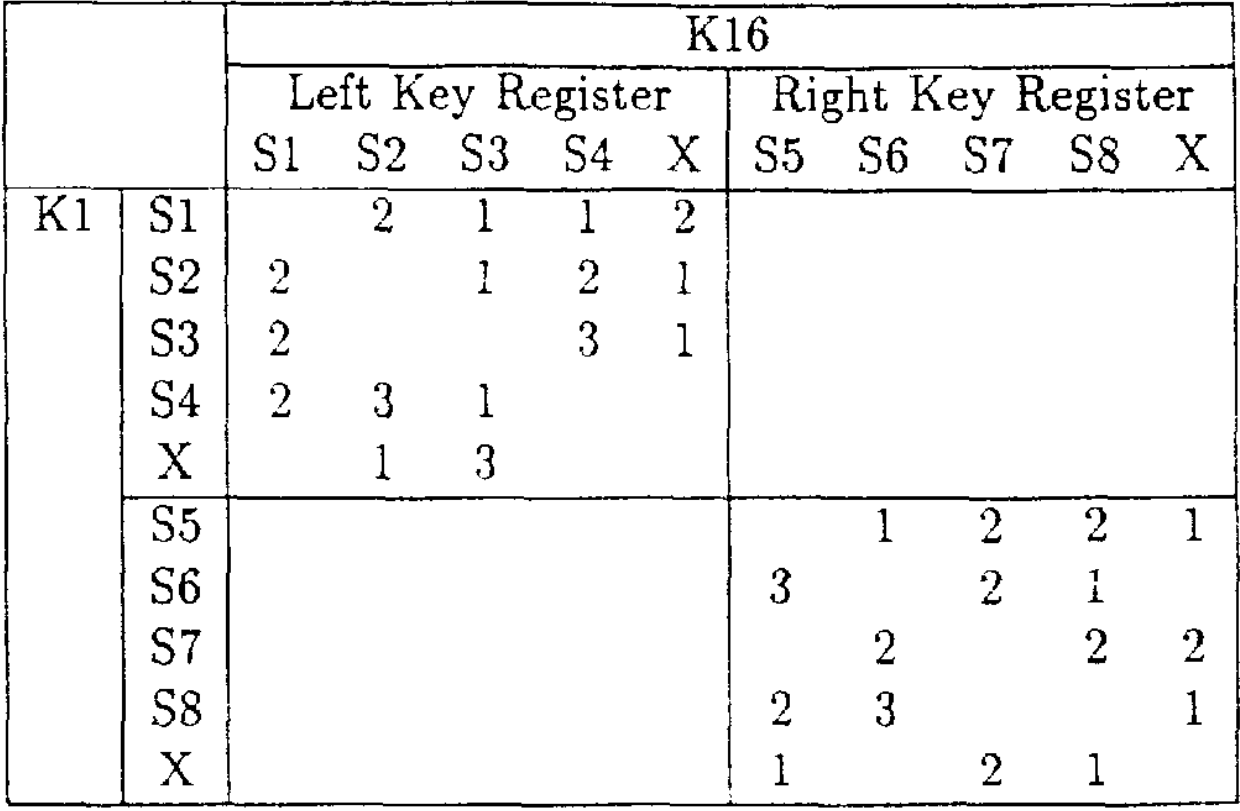
\includegraphics[width=\columnwidth]{images/des-k1-k16.png}
                    \caption{Common bits between \(K1\) and \(K16\).}
                    \label{fig:des-k1-k16}
                \end{figure}
            \end{column}
        \end{columns}
    \end{frame}

    \subsection{Results}
    \label{subsec:results}

    \begin{frame}
        \frametitle{General Form of the Attack}
        \begin{theorem}
        \label{thm:gen-attack}    
        Given a characteristic with probability \(p\) and signal-to-noise ratio
        \(S/N\) for an iterated cryptosystem with \(k\) key bits, we can apply
        an attack which encrypts \(\frac{2}{p}\) chosen plaintexts in the data
        collection phase and whose complexity is \(\frac{2^k}{S/N}\) encryptions
        during the data analysis phase.
        \end{theorem}
        
        \visible<2->{Appropriately chosen metastructures can reduce the number
        of plaintexts to \(\frac{1}{p}\). Further, the effective time complexity
        can be reduced by a factor of \(f \le 1\) if a wrong key can be
        discarded by carrying out a fraction \(f\) of the rounds.}
    \end{frame}
    

    \begin{frame}
        \frametitle{Results}
        \begin{figure}[!ht]
            \centering
            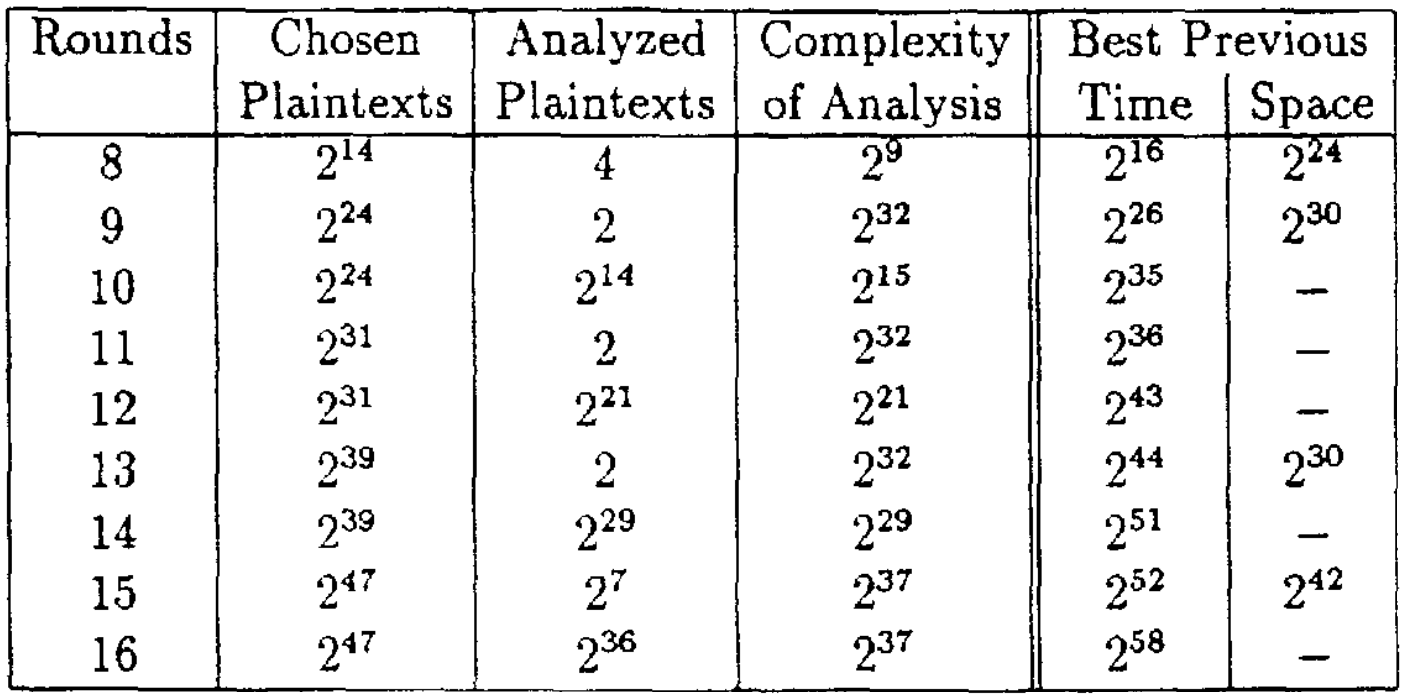
\includegraphics[width=0.7\linewidth]{images/summary_new.png}
            \caption{Results of memoryless DES attack.}
            \label{fig:des-new-summary}
        \end{figure}
    \end{frame}
\end{document}